%% Produit par outils/generer_tonalites.py — ne pas modifier à la main.
\textbf{1.} ré majeur~:~si mineur, la majeur, fa dièse mineur, sol majeur, mi mineur~; mi bémol majeur~:~do mineur, si bémol majeur, sol mineur, la bémol majeur, fa mineur~; si mineur~:~ré majeur, fa dièse mineur, la majeur, mi mineur, sol majeur~; fa mineur~:~la bémol majeur, do mineur, mi bémol majeur, si bémol mineur, ré bémol majeur.

\textbf{2.} En fa majeur, un bémol à l'armure ; le do bécarre de la mesure~2 devient mi bémol.

\begin{center}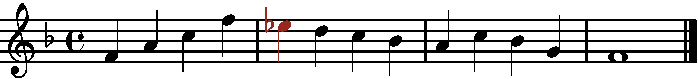
\includegraphics[width=0.8\linewidth]{t-exercice-reponse.cropped.pdf}\end{center}

\textbf{3.} 1~:~sol mixolydien, les notes de do majeur~; 2~:~la dorien, les notes de sol majeur~; 3~:~ré lydien, les notes de la majeur~; 4~:~do phrygien, les notes de la bémol majeur.
